\section{Dynamic 3-Armed Bandit}
\label{task:flux}

\textbf{Action values vary with time within each trial, independently across arms}

\begin{figure}[h]%
    \centering
    \subfloat{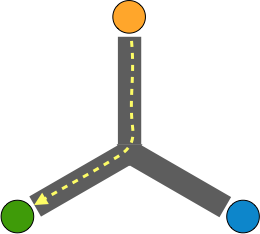
\includegraphics[width=0.25\textwidth]{flux/3arm_scheme.png}}%
    \qquad
    \subfloat{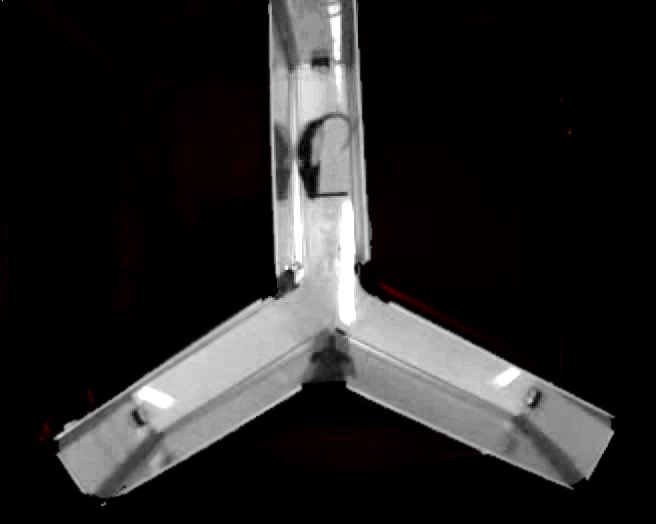
\includegraphics[width=0.25\textwidth]{flux/maze2-filtered-1587.jpeg}}%
    \caption{Maze scheme and picture}%
    \label{fig:3arm}%
\end{figure}

In this task, rats move freely within a 3-arm maze (figure \ref{fig:3arm}) collecting water rewards at spouts located at the end of each arm (one spout per arm).
Rewards are delivered if a spout is visited and at least $\iota$ seconds have elapsed since the last occurrence of a reward at that same spout.
Interval $\iota$ takes different values for each of the 3 arms ($\iota_{\text{arm}}$), and in different sessions (or task variants) is either an exponentially distributed random variable (a different mean for each arm, fixed within a session) or a constant (different for each arm, fixed within a session)\footnote{These variants are known in experimental psychology as concurrent variable and fixed interval schedules of reinforcement, respectively (e.g. Herrnstein's Matching law paper \cite{herrnstein1961relative}.)}

In the case of $\iota \sim Exp(\lambda)$ and for any given arm, the probability of reward when checking the spout at time $t$ (relative to last reward at that same arm) is simply the CDF of $\iota$ evaluated at $t$: $P(r \mid t) = 1 - e^{-\lambda t}$.

Thus, reward probabilities at each of the 3 spouts (action values) can be simply and precisely computed at any given moment, and it is plausible that animals could approximate a reward maximizing strategy based on those estimates.
Alternatively, animals might employ a simplified strategy that discards action value dynamics, instead learning scalar representations of action values.
These alternative strategies are illustrated by the two following RL models (adapted from \cite{constantino2015learning}):

\textbf{(Model 1, scalar action values)}
This is a simple model-free RL agent learning scalar, cached action values relative to average reward rate (R-learning).
Action values were initialized randomly, and decisions made based on a softmax rule.
Each choice implied committing to that option for a certain amount of time - a longer "travel time" if switching arms, or a shorter "harvest time" for repeated choices.
Rewards were delivered according to the task rule described above.

\begin{figure}%
    \centering
    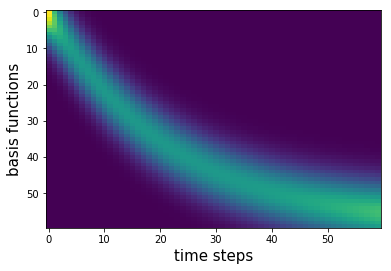
\includegraphics[width=0.35\textwidth]{flux/microStimuli.png}%
    \caption{Temporal basis functions used to represent time varying action values. RL agent of model 2 learned a linear readout vector for each action. Time is relative to last reward at same arm for which action value is being computed.}
    \label{fig:basisFun}%
\end{figure}

\textbf{(Model 2, time varying action values)}
This model is similar to model 1, differing only in that instead of learning a scalar for each action, the agent learned a linear readout vector used to compute the action values from the basis functions depicted in figure \ref{fig:basisFun}.

Both simulated agents chose among the 3 arms in proportion to rewards obtained from each arm (figure \ref{fig:flux_model}, top row), thus conforming to the Matching law \cite{herrnstein1961relative}.
In other words, matching behavior fails to distinguish between the two very different behavioral strategies embodied in models 1 and 2.
The rat also displayed matching ("data" in figure \ref{fig:flux_model}).

Lastly, a logistic regression was used to assess the dependence of choice of arm on time since last rewards on each arm.
Model 1 learns a scalar value for each action (inset in figure \ref{fig:flux_model}, bottom left), but as expected choices are not time dependent.
Model 2 learns a time varying value for each action (inset in figure \ref{fig:flux_model}, bottom center), and as expected choices are indeed time dependent.
While we cannot directly read action value representations from the rat, we were indeed able to predict its choices based on time since last rewards, thus suggesting that animals keep track of time varying reward probabilities.

\begin{figure}%
    \centering
    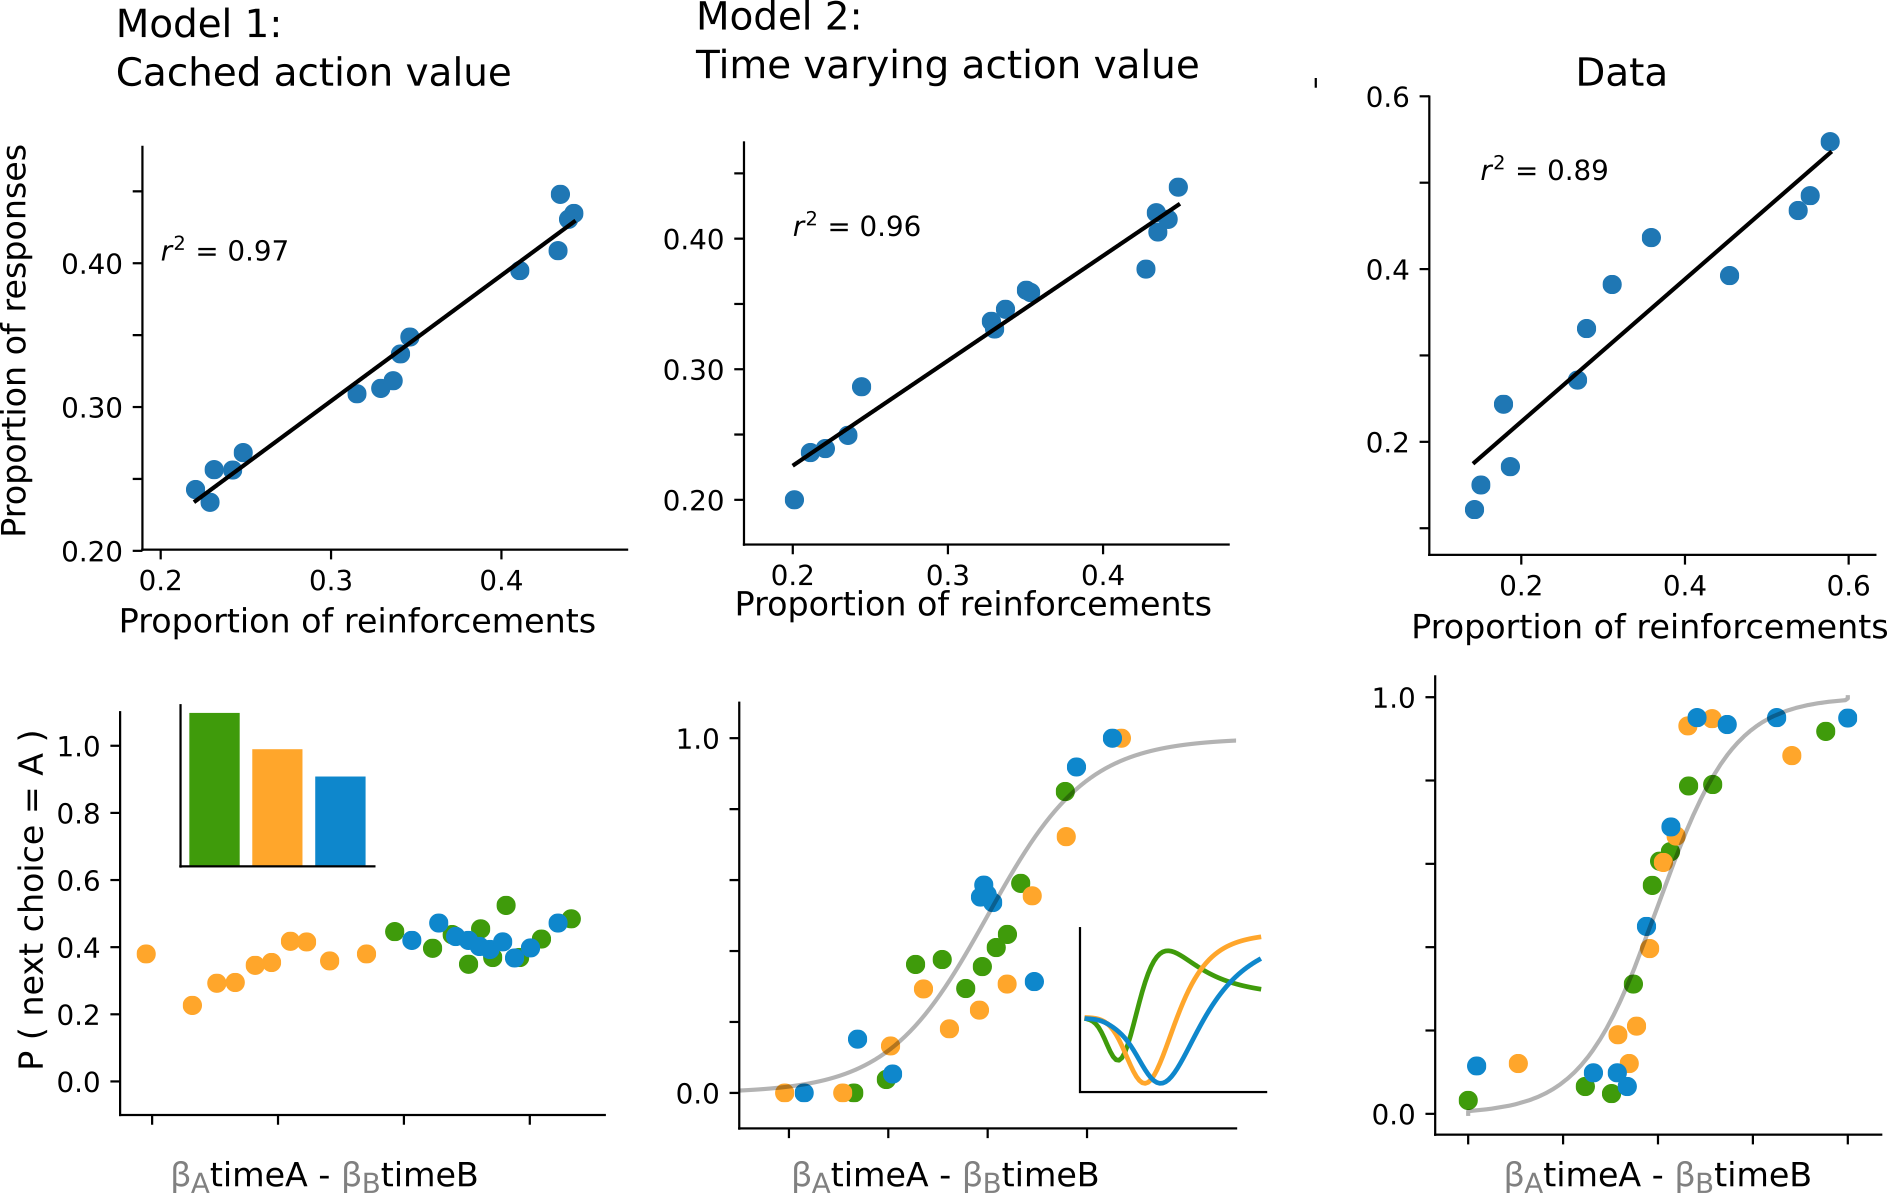
\includegraphics[width=0.7\textwidth]{flux/02_model.png}%
    \caption{Qualitative comparison between scalar vs time varying action value models (1 and 2, respectively) and data. Top row: proportion of choices matches proportion of rewards for all three agents. Bottom row: logistic regression predicts what arm will be visited next based on time elapsed since last reward at each of the two alternatives (color: arm of origin; insets: action values). As expected, time predicts next choice for model 2, but not for model 1. Data resemble model 2, suggesting animals keep track of time varying action values.}
    \label{fig:flux_model}%
\end{figure}

% [flat hazard rate]